\section{MSVC: \RU{Пример SYSTEMTIME}\EN{SYSTEMTIME example}}
\label{sec:SYSTEMTIME}

\newcommand{\FNSYSTEMTIME}{\footnote{\href{http://msdn.microsoft.com/en-us/library/ms724950(VS.85).aspx}{MSDN: SYSTEMTIME structure}}}

\RU{Возьмем, к примеру, структуру SYSTEMTIME\FNSYSTEMTIME{} из win32 описывающую время.}
\EN{Let's take SYSTEMTIME\FNSYSTEMTIME{} win32 structure describing time.}

\RU{Она объявлена так:}\EN{That's how it is defined:}

\begin{lstlisting}[caption=WinBase.h]
typedef struct _SYSTEMTIME {
  WORD wYear;
  WORD wMonth;
  WORD wDayOfWeek;
  WORD wDay;
  WORD wHour;
  WORD wMinute;
  WORD wSecond;
  WORD wMilliseconds;
} SYSTEMTIME, *PSYSTEMTIME;
\end{lstlisting}

\RU{Пишем на Си функцию для получения текущего системного времени:}
\EN{Let's write a C function to get current time:}

\lstinputlisting{patterns/15_structs/systemtime.c}

\RU{Что в итоге}\EN{We got} (MSVC 2010):

\lstinputlisting[caption=MSVC 2010 /GS-]{patterns/15_structs/systemtime.asm}

\RU{Под структуру в стеке выделено 16 байт ~--- именно столько будет \TT{sizeof(WORD)*8}
(в структуре 8 переменных с типом WORD).}
\EN{16 bytes are allocated for this structure in local stack~---that is exactly \TT{sizeof(WORD)*8}
(there are 8 WORD variables in the structure).}

\newcommand{\FNMSDNGST}{\footnote{\href{http://msdn.microsoft.com/en-us/library/ms724390(VS.85).aspx}{MSDN: GetSystemTime function}}}

\RU{Обратите внимание на тот факт, что структура начинается с поля \TT{wYear}. 
Можно сказать, что в качестве аргумента для \TT{GetSystemTime()}\FNMSDNGST передается указатель на структуру 
SYSTEMTIME, но можно также сказать, что передается указатель на поле \TT{wYear}, 
что одно и тоже! 
\TT{GetSystemTime()} пишет текущий год в тот WORD на который указывает переданный указатель, 
затем сдвигается на 2 байта вправо, пишет текущий месяц, и т.д., и т.д.}
\EN{Pay attention to the fact the structure beginning with \TT{wYear} field.
It can be said, an pointer to SYSTEMTIME structure is passed to the \TT{GetSystemTime()}\FNSYSTEMTIME,
but it is also can be said, pointer to the \TT{wYear} field is passed, and that is the same!
\TT{GetSystemTime()} writes current year to the WORD pointer pointing to, then shifts 2 bytes
ahead, then writes current month, etc, etc.}

\subsection{\olly}
\index{\olly}

\RU{Компилируем этот пример в}\EN{Let's compile this example in} MSVC 2010 \RU{с ключами}\EN{with} 
\TT{/GS- /MD} \RU{и запускаем в}\EN{keys and run it in} \olly.
\RU{Открываем окна данных и стека по адресу, который передается в качестве первого аргумента в ф-цию}
\EN{Let's open windows of data and stack at the address which is passed as the first argument into}
\TT{GetSystemTime()}\EN{ function}, 
\RU{ждем пока эта ф-ция исполнится, и видим следующее}\EN{let's wait until it's executed and we see this}:
\figname \ref{fig:struct_olly_1}.

\RU{Точное системнео время на моем компьютере, в которое исполнилась ф-ция, это}
\EN{Precise system time of function execution on my computer is} 5 \RU{июня}\EN{june} 2014, 7:17:45:
\figname \ref{fig:struct_olly_2}.

\RU{Таким образом, в окне данных мы видим следующие 16 байт}\EN{So we see these 16 bytes in the
data window}: 
\begin{lstlisting}
DE 07 06 00 04 00 04 00
07 00 11 00 2D 00 8D 00
\end{lstlisting}

\RU{Каждые два байта отражают одно поле структуры}\EN{Each two bytes representing one structure field}. 
\RU{А так как порядок байт (\gls{endianness}) \IT{little endian},
то в начале следует младший байт, затем старший}\EN{Since \gls{endianness} is \IT{little endian}, 
we see low byte first and then high one}.
\RU{Следовательно, вот какие 16-битные числа сейчас записаны в памяти}
\EN{Hence, these are values which are currently stored in memory}:

\begin{center}
\begin{tabular}{ | l | l | l | }
\hline
\headercolor{} \RU{Шестнадцатиричное число}\EN{Hexadecimal number} & 
\headercolor{} \RU{десятичное число}\EN{decimal number} & 
\headercolor{} \RU{имя поля}\EN{field name} \\
\hline
0x07DE & 2014	& wYear \\
\hline
0x0006 & 6	& wMonth \\
\hline
0x0004 & 4	& wDayOfWeek \\
\hline
0x0005 & 5	& wDay \\
\hline
0x0007 & 7	& wHour \\
\hline
0x0011 & 17	& wMinute \\
\hline
0x002D & 45	& wSecond \\
\hline
0x008D & 141	& wMilliseconds \\
\hline
\end{tabular}
\end{center}

\RU{В окне стека, видны те же значения, только они сгруппированы как 32-битные значения}
\EN{The same values are seen in the stack window, but they are groupped as 32-bit values}.

\RU{Затем}\EN{And then} \printf \RU{просто берет нужные значения и выводит их на консоль}
\EN{just takes values it needs and outputs them to the console}.

\RU{Некоторые поля}{Some values} \printf \RU{не выводит}{doesn't output} (\TT{wDayOfWeek} \AndENRU 
\TT{wMilliseconds}), \RU{но они находятся в памяти и доступны для использования}{but they are
in memory right now, available for using}.

\begin{figure}[H]
\centering
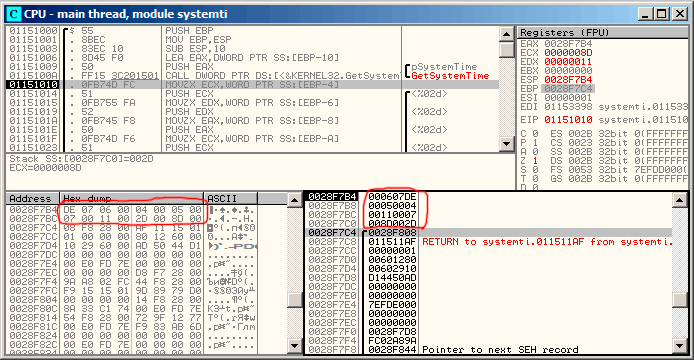
\includegraphics[scale=\FigScale]{patterns/15_structs/olly_systemtime1.png}
\caption{\olly: \TT{GetSystemTime()} \RU{только что исполнилась}\EN{just executed}}
\label{fig:struct_olly_1}
\end{figure}

\begin{figure}[H]
\centering
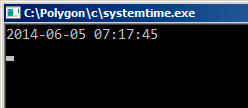
\includegraphics[scale=0.66]{patterns/15_structs/olly_systemtime2.png}
\caption{\olly: \RU{Вывод \printf}\EN{\printf output}}
\label{fig:struct_olly_2}
\end{figure}

\subsection{\RU{Замена структуры массивом}\EN{Replacing the structure by array}}

\RU{Тот факт, что поля структуры это просто переменные расположенные рядом, 
я могу проиллюстрировать следующим образом.}
\EN{The fact the structure fields are just variables located side-by-side, 
I can demonstrate by the following technique.}
\RU{Глядя на описание структуры}\EN{Keeping in ming} \TT{SYSTEMTIME}
\RU{, я могу переписать этот простой пример так:}
\EN{ structure description, I can rewrite this simple example like this:}

\lstinputlisting{patterns/15_structs/systemtime2.c}

\RU{Компилятор немного поворчит:}\EN{Compiler will grumble for a little:}

\begin{lstlisting}
systemtime2.c(7) : warning C4133: 'function' : incompatible types - from 'WORD [8]' to 'LPSYSTEMTIME'
\end{lstlisting}

\RU{Тем не менее, выдаст такой код}\EN{But nevertheless, it will produce this code}:

\lstinputlisting[caption=MSVC 2010]{patterns/15_structs/systemtime2.asm}

\RU{И это работает так же}\EN{And it works just as the same}!

\RU{Любопытно что результат на ассемблере неотличим от предыдущего}
\EN{It is very interesting fact the
result in assembly form cannot be distinguished from the result of previous compilation}.
\RU{Таким образом, глядя на этот код, 
никогда нельзя сказать с уверенностью, была ли там объявлена структура, либо просто набор переменных.}
\EN{So by looking at this code, one cannot say for sure, was there structure declared, or just pack of variables.} 

\RU{Тем не менее, никто в здравом уме делать так не будет}
\EN{Nevertheless, no one will do it in sane state of mind}.
\RU{Потому что это неудобно}\EN{Since it is not convenient}. 
\RU{К тому же, иногда, поля в структуре могут меняться разработчиками, 
переставляться местами, и т.д}\EN{Also structure fields may be changed by developers, swapped, etc}.

\RU{Я не привожу здесь пример с \olly, потому что он будет точно такой же, как и в случае со структурой.}
\EN{I'm not adding \olly example here, because it will be just as the same as in the case 
with structure.}

